\documentclass[main]{subfiles}

\begin{document}
	\subsection{Площадь поверхности (без доказательства). Контрпример Шварца}

	\begin{theorem}
  	    Площадь поверхности $S = \iint\limits_D \sqrt{EG - F^2} du dv$
  	    %картинка про площадь
	\end{theorem}

	\begin{example}[контрпример]
		Как не нужно вводить площадь?\\
		Конструкция: Ф --- пов-ть, впишем в Ф  кус.-лин. пов-ть
		\[\lim_{|\Delta_i| \ra 0} \sum_{\Delta} S_{\Delta} \os{?}{=} S_{\text{пов-ти}}\]
		\begin{figure}[H]
			\centering
			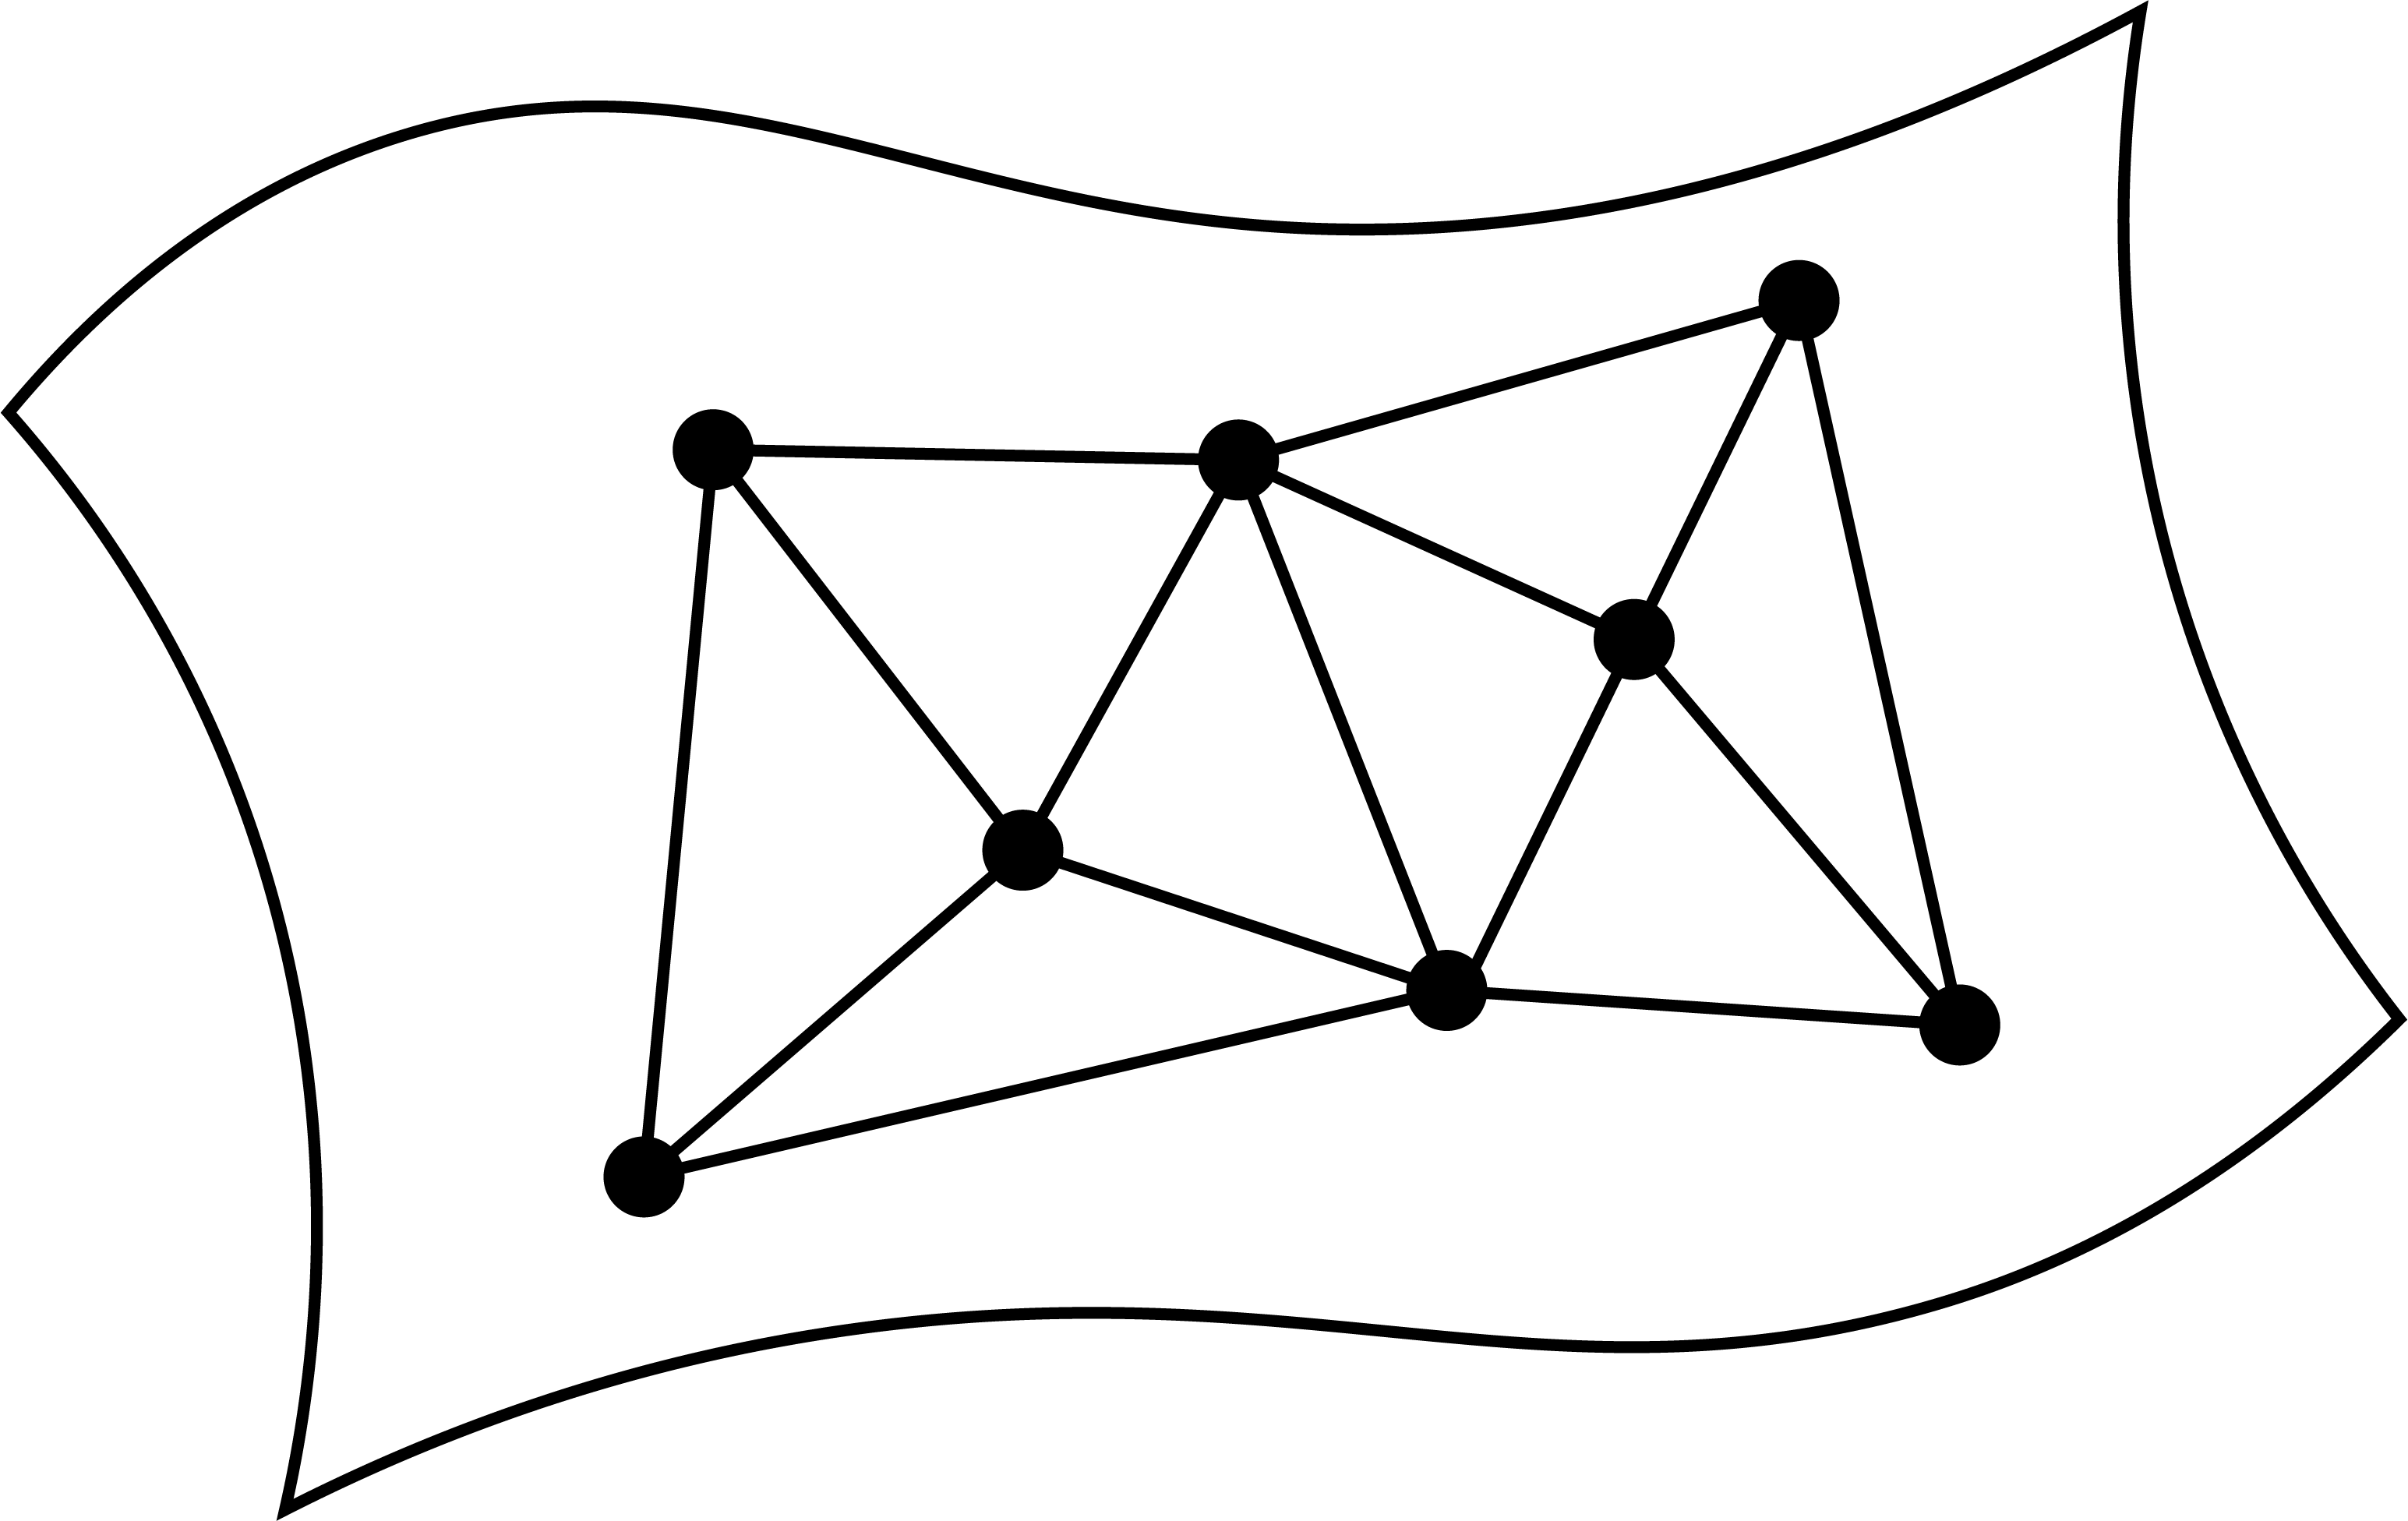
\includegraphics[width=5cm]{pics/7_1.png}
		\end{figure}
		Контрпример: сапог Шварца\\
		\begin{figure}[H]
			\centering
			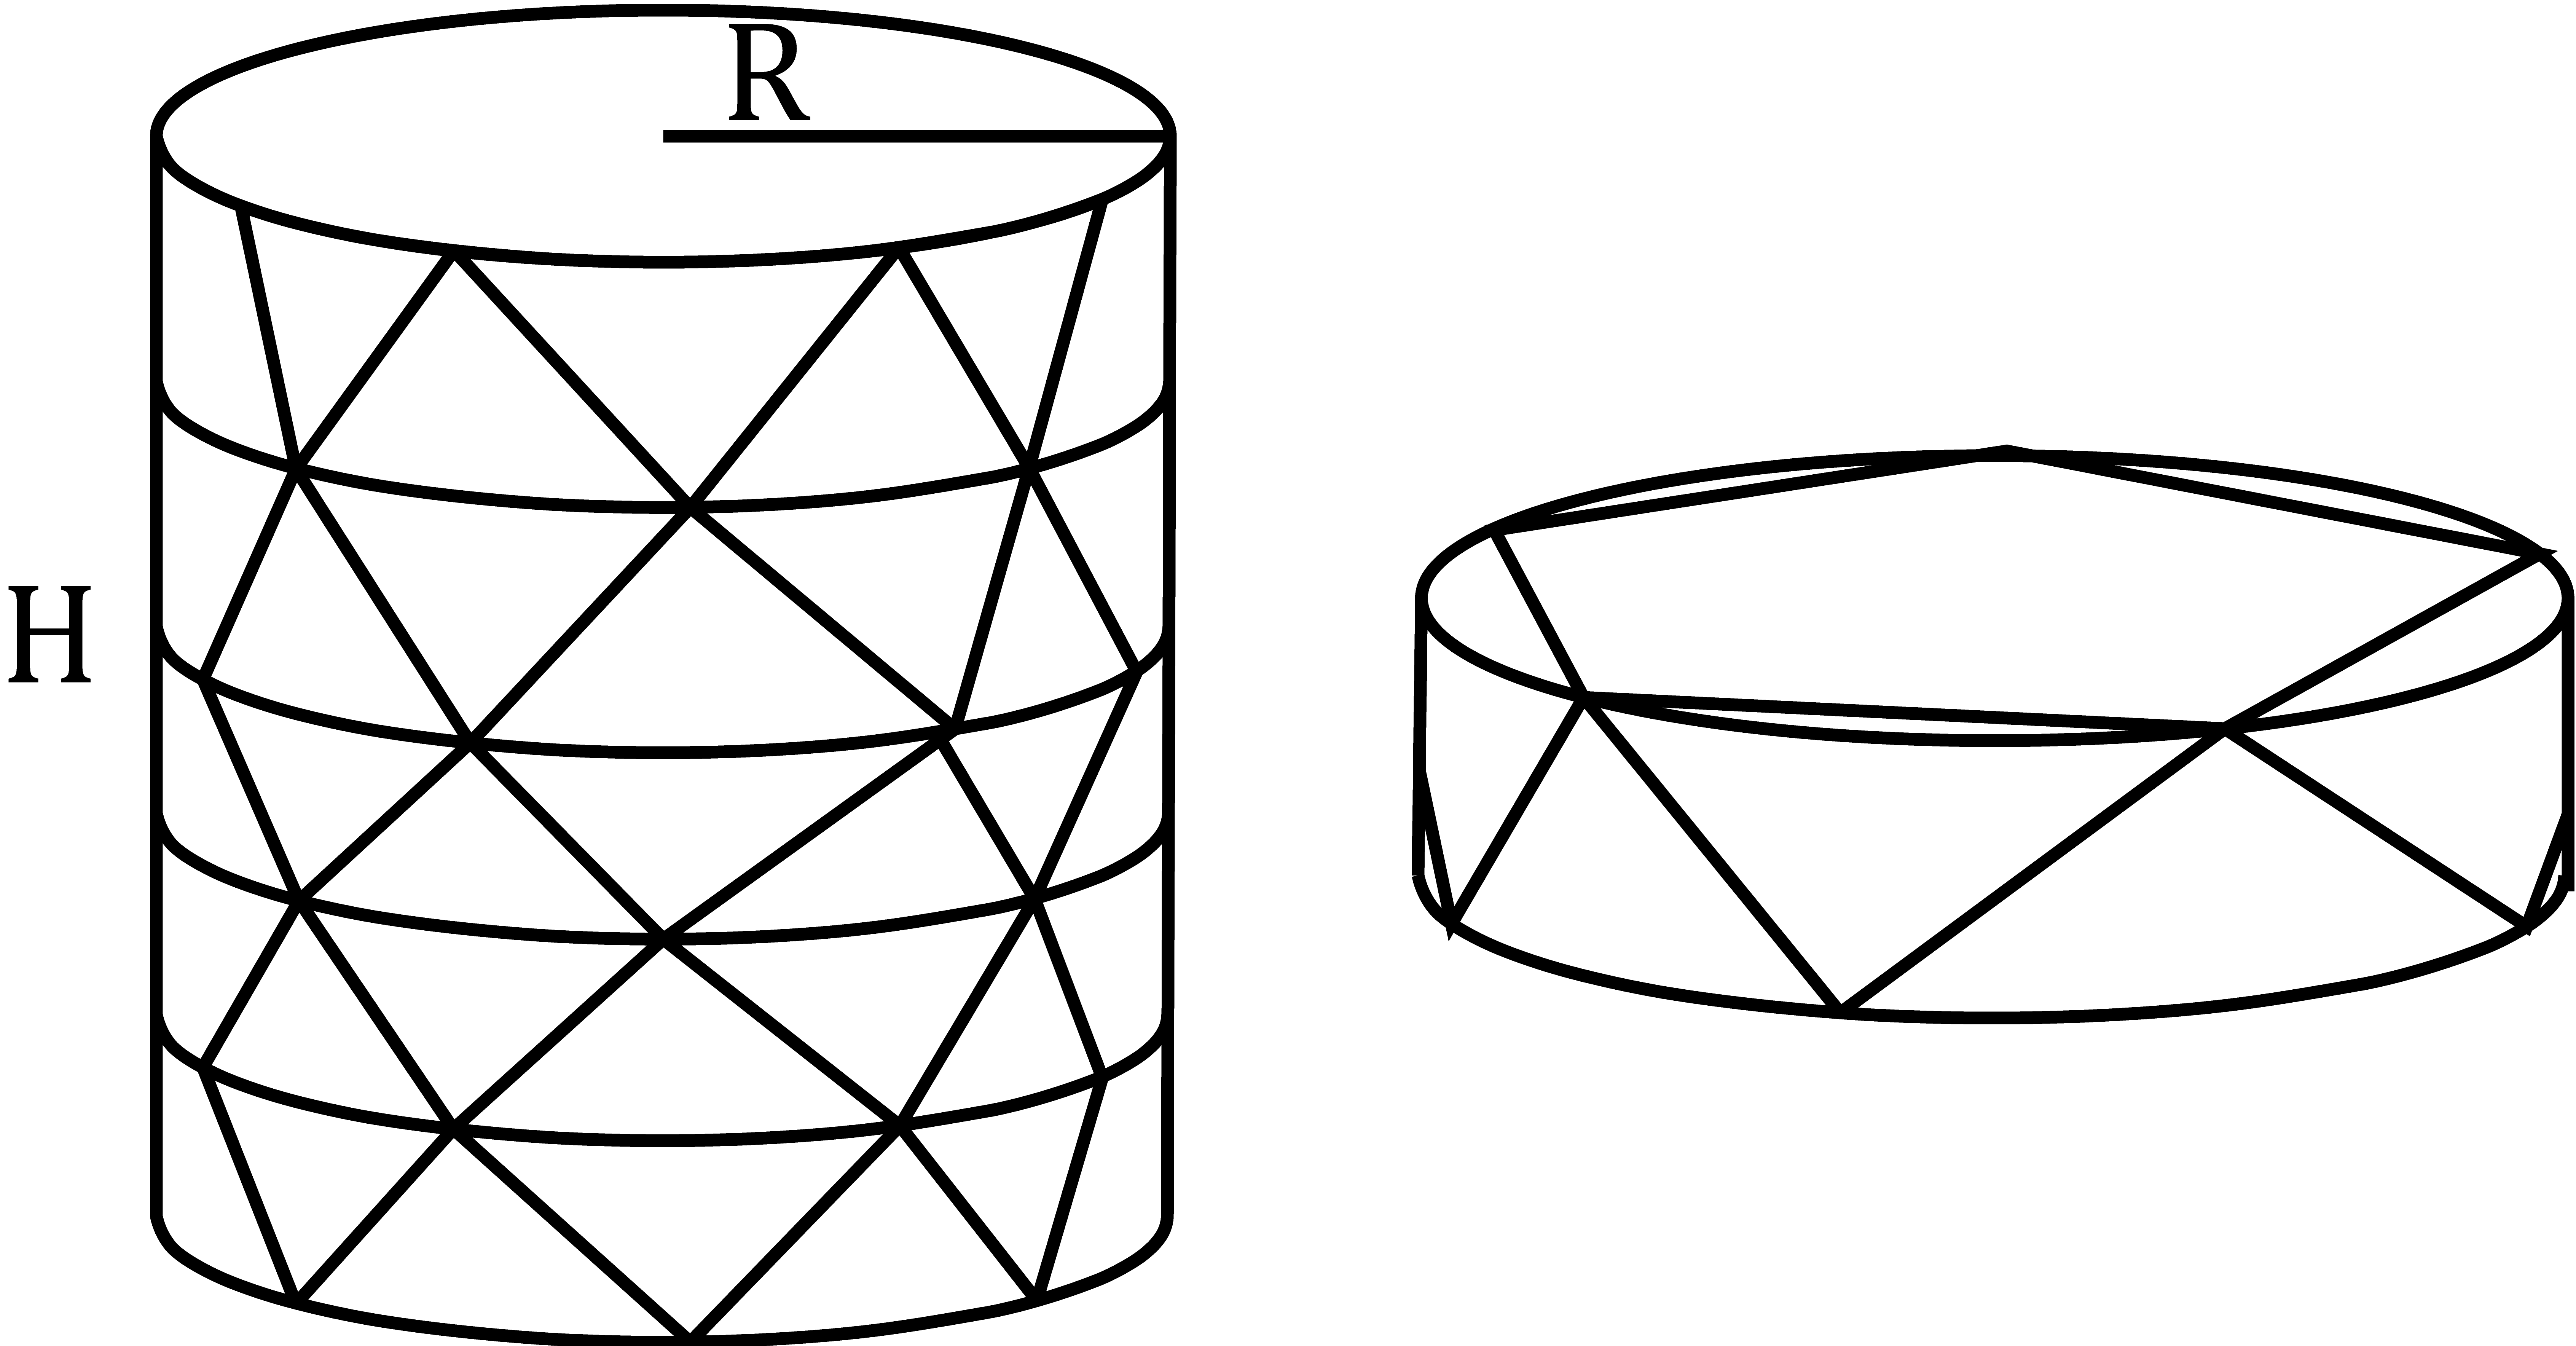
\includegraphics[width=7cm]{pics/7_2.png}
		\end{figure}

		$h$ --- высота каждого\\
		$k$ слоев
		\[H = k h\]
		\[k,n \ra \infty\]
		\begin{figure}[H]
			\centering
			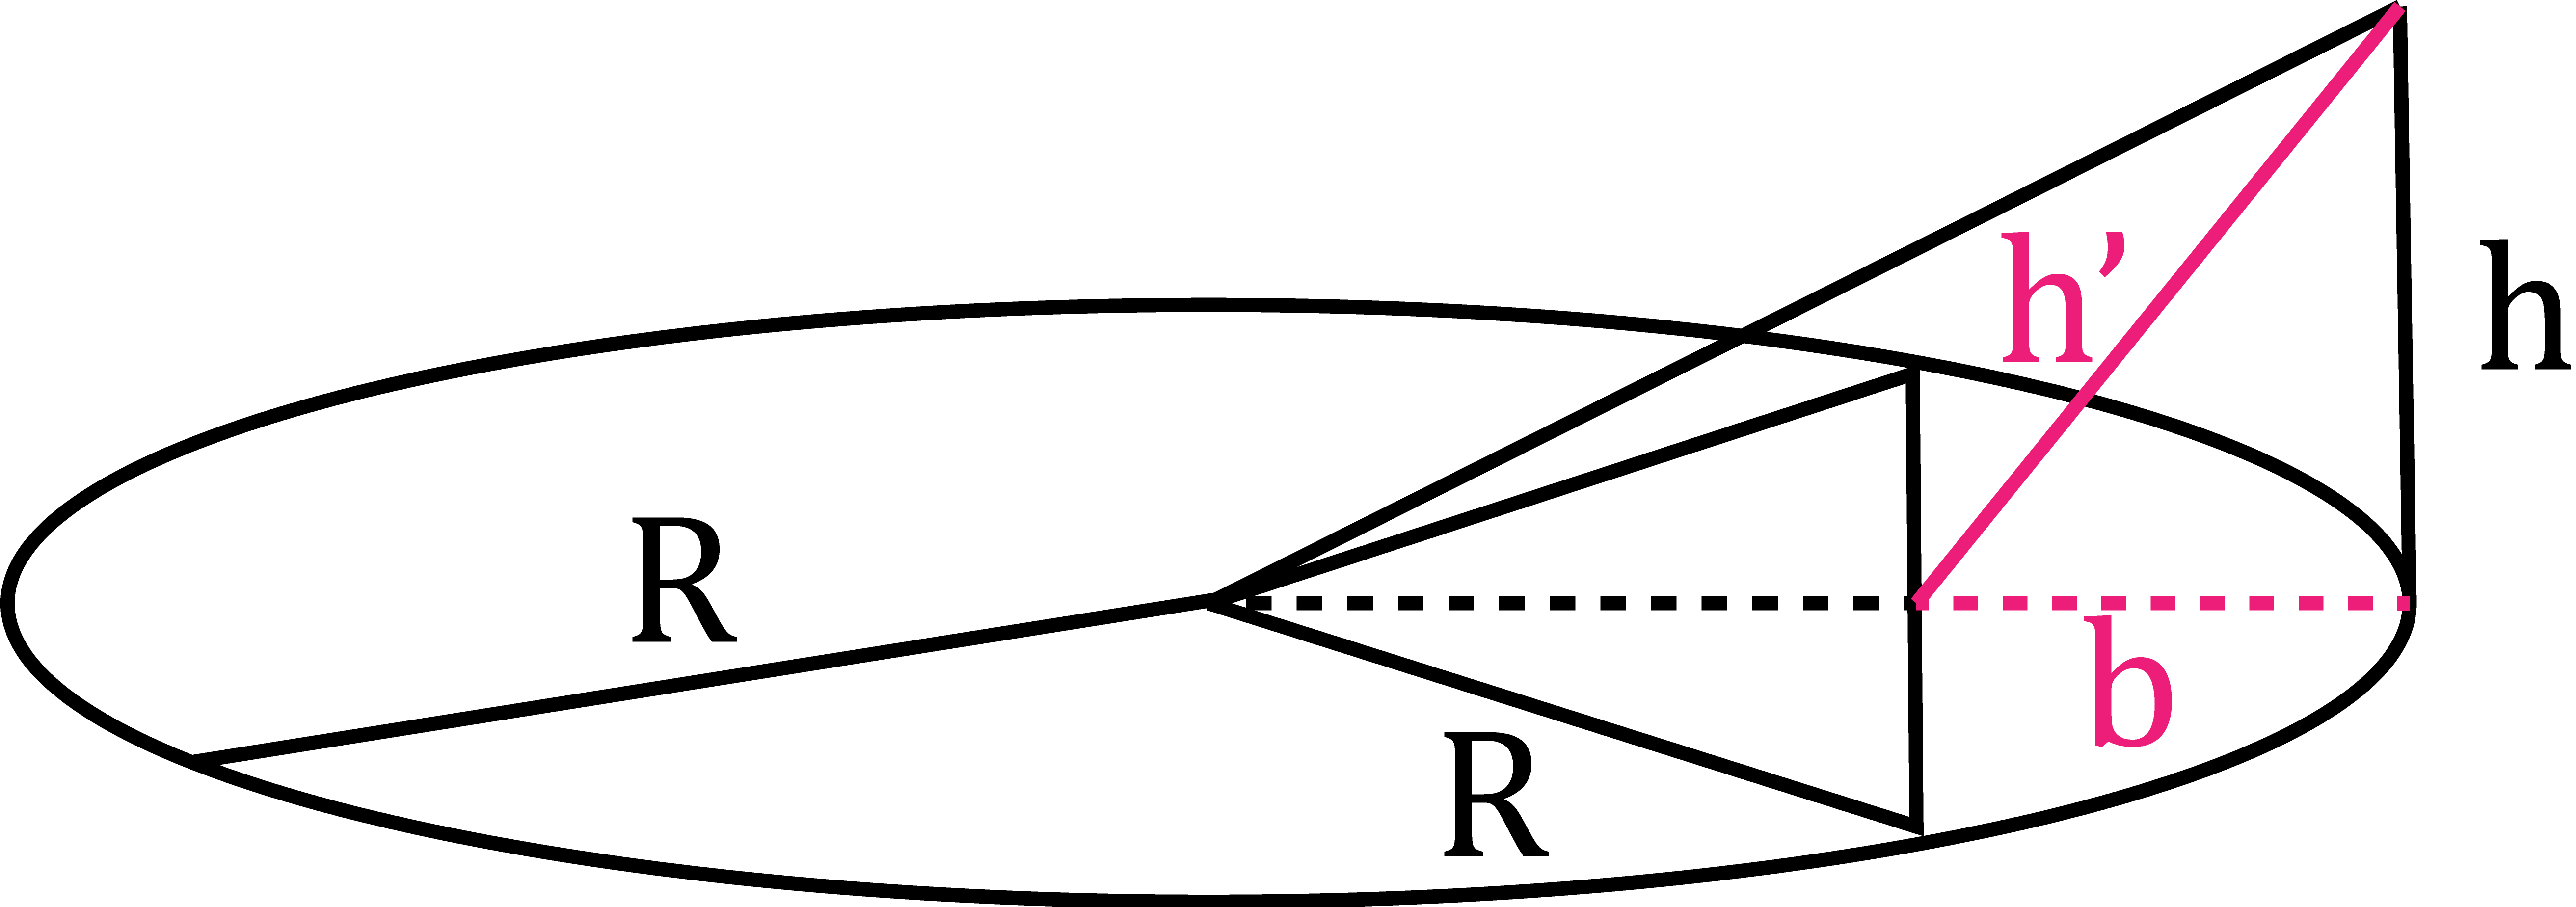
\includegraphics[width=6cm]{pics/7_3.png}
		\end{figure}
		В слое 2n $\Delta$
		\[h'=\sqrt{h^2 + b^2}\]
		Всего 2nk $\Delta$
		\begin{figure}[H]
			\centering
			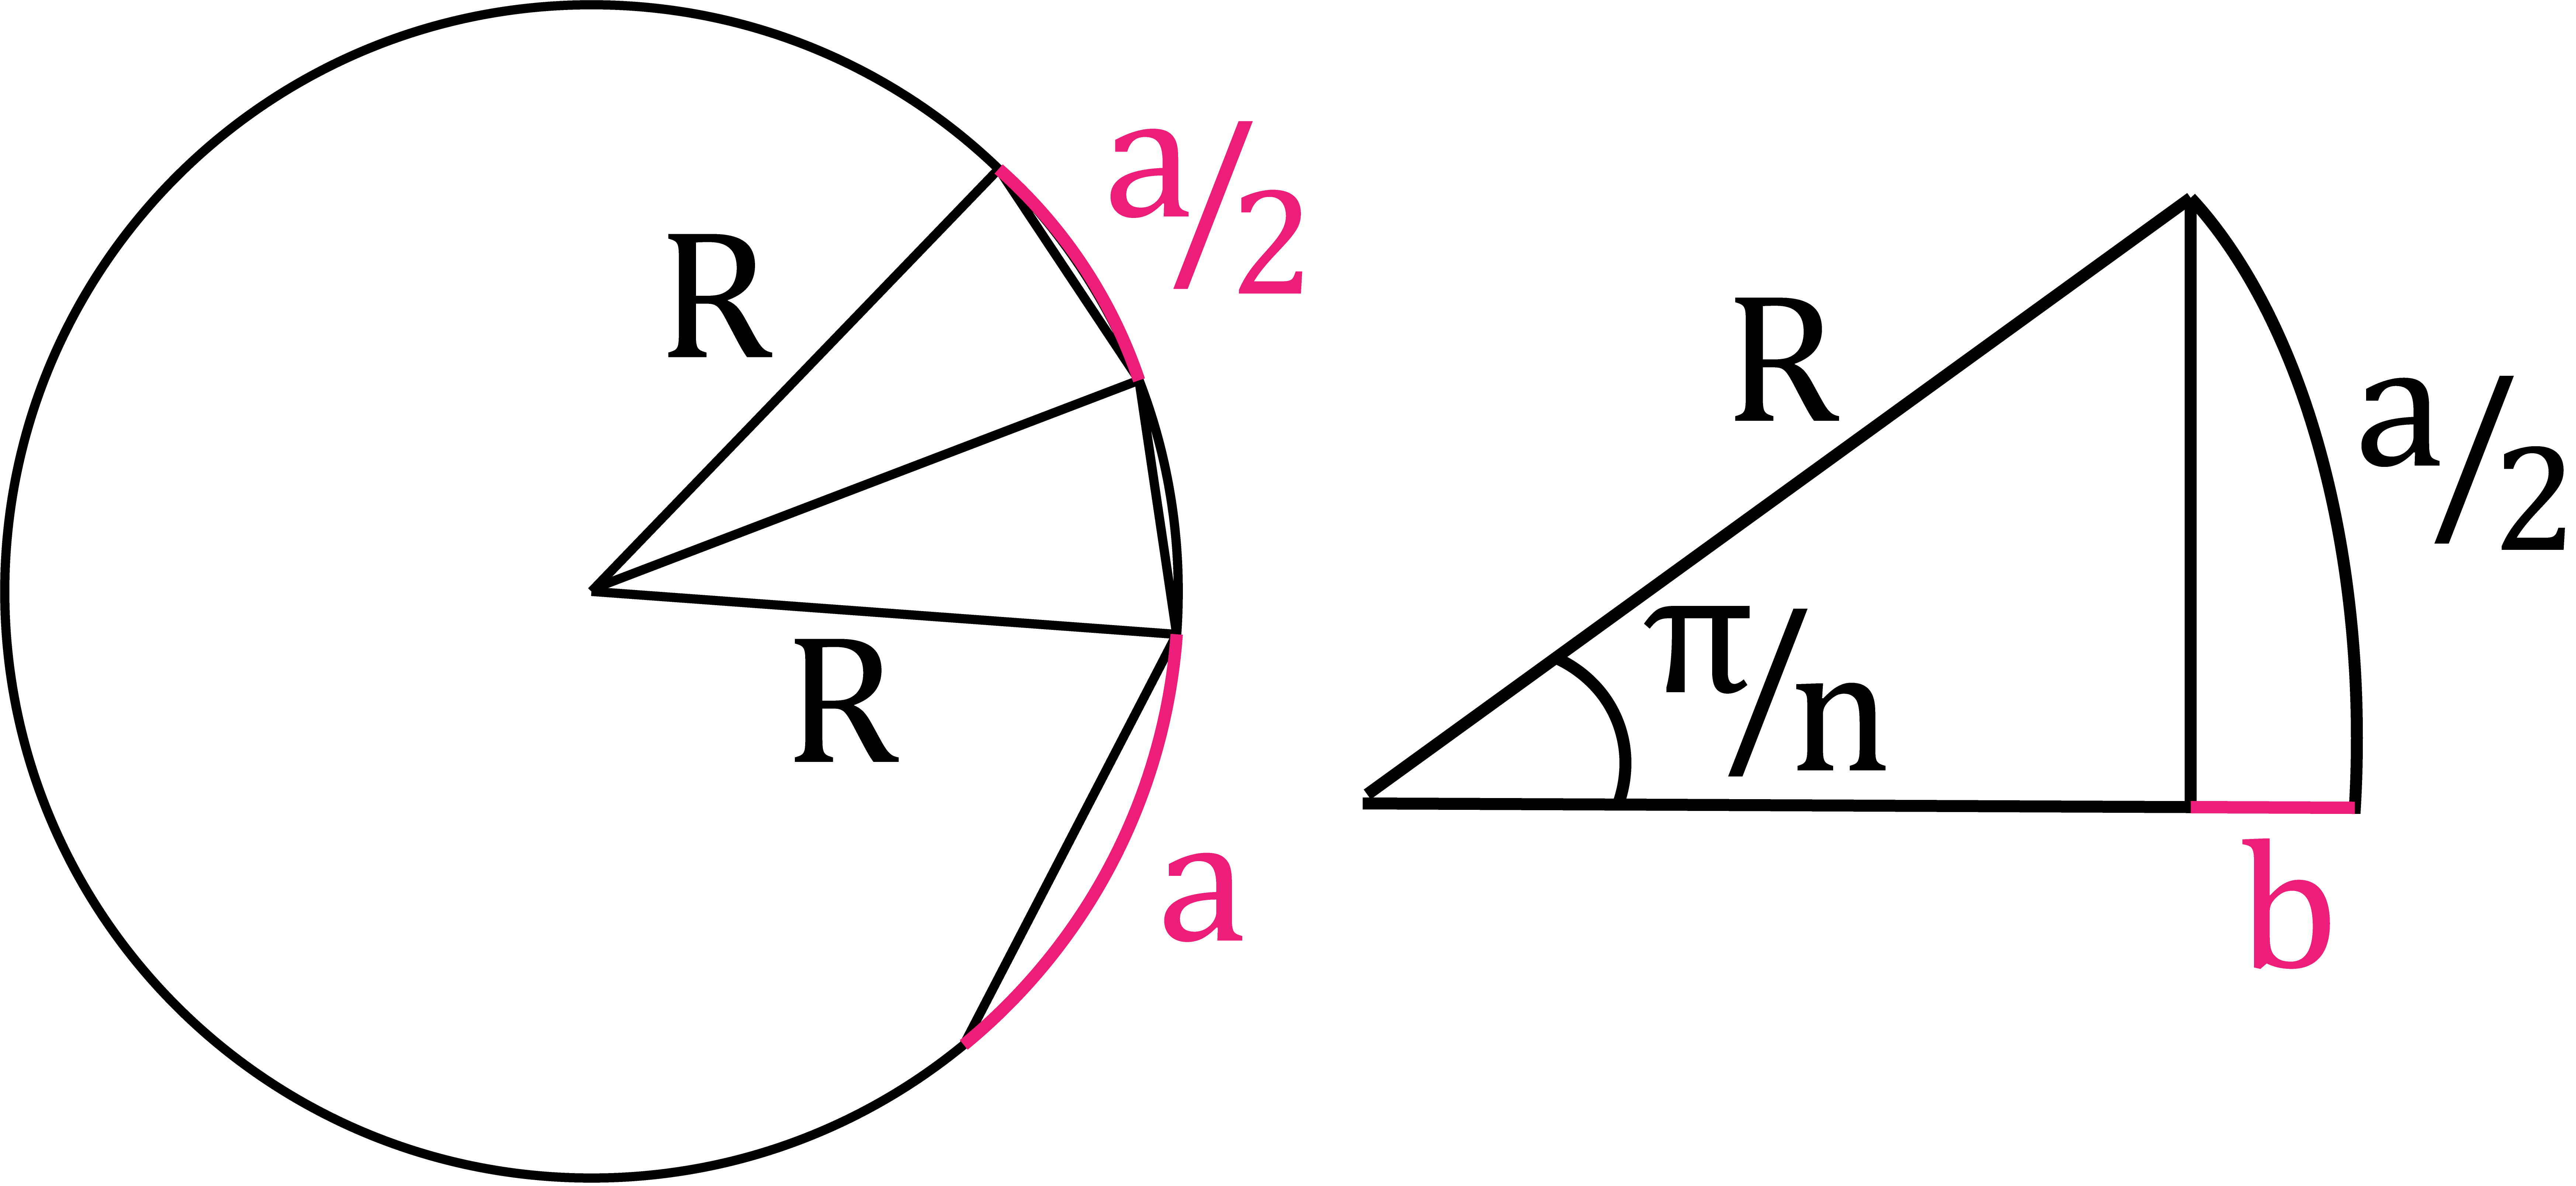
\includegraphics[width=8cm]{pics/7_4.png}
		\end{figure}
		\[\dfrac{a}{2} = R \sin \dfrac{\pi}{n}\]
		\[a = 2 R \sin \dfrac{\pi}{n}\]
		\[b = R - R \cos \dfrac{\pi}{n} \q h = \dfrac{H}{K}\]
		\[h' = \sqrt{h^2 + R^2 (1-\cos \dfrac{\pi}{n})^2}\]
		\[S = \dfrac{1}{2} a h' = R \sin \dfrac{\pi}{n} \sqrt{h^2 + R^2 (1-\cos \dfrac{\pi}{n})^2}\]

		\[\sum_{\Delta} S_{\Delta} = 2nk R \sin \dfrac{\pi}{n} \sqrt{\dfrac{H^2}{k^2} + R^2 (1-\cos \dfrac{\pi}{n})^2}\]
		\begin{multline*}
			\lim_{n,k \ra \infty} 2nk R \sin \dfrac{\pi}{n} \sqrt{\dfrac{H^2}{k^2} + R^2 (1-\cos \dfrac{\pi}{n})^2} = \\
			\qq \qq = 2 \pi R \lim_{n,k \ra \infty} \sqrt{H^2 + R^2 (1-\cos \dfrac{\pi}{n})^2 k^2} = \\
			\qq \qq \qq \qq = 2 \pi R \sqrt{H^2 + R^2 \lim_{n,k \ra \infty} k^2 (1-\cos \dfrac{\pi}{n})^2} = \\
			= 2\pi R \sqrt{H^2 + R^2 \dfrac{\pi^4}{4} \lim_{k,n \ra \infty} \dfrac{k^2}{n^4}}
		\end{multline*}
		Если $k=\us{n \ra \infty}{o(n^2)} \Ra 2\pi RH$\\
		Если $k = n^2 \Ra 2 \pi R \sqrt{H^2 + \dfrac{\pi^4}{4} R^2} \neq 2\pi R H$\\
		Если $k = n^3 \Ra ... = \infty$\\ \\
		Почему так? \\
		Посмотрим, что происходит, когда k растет быстрее, чем $n^2$\\
		При маленьком a выходит тонкий слой и получается "помятый"{} сапог Шварца
	\end{example}

	\subsection{Кривизна кривой на поверхности. Вторая квадратичная форма}
	\begin{figure}[H]
		\centering
		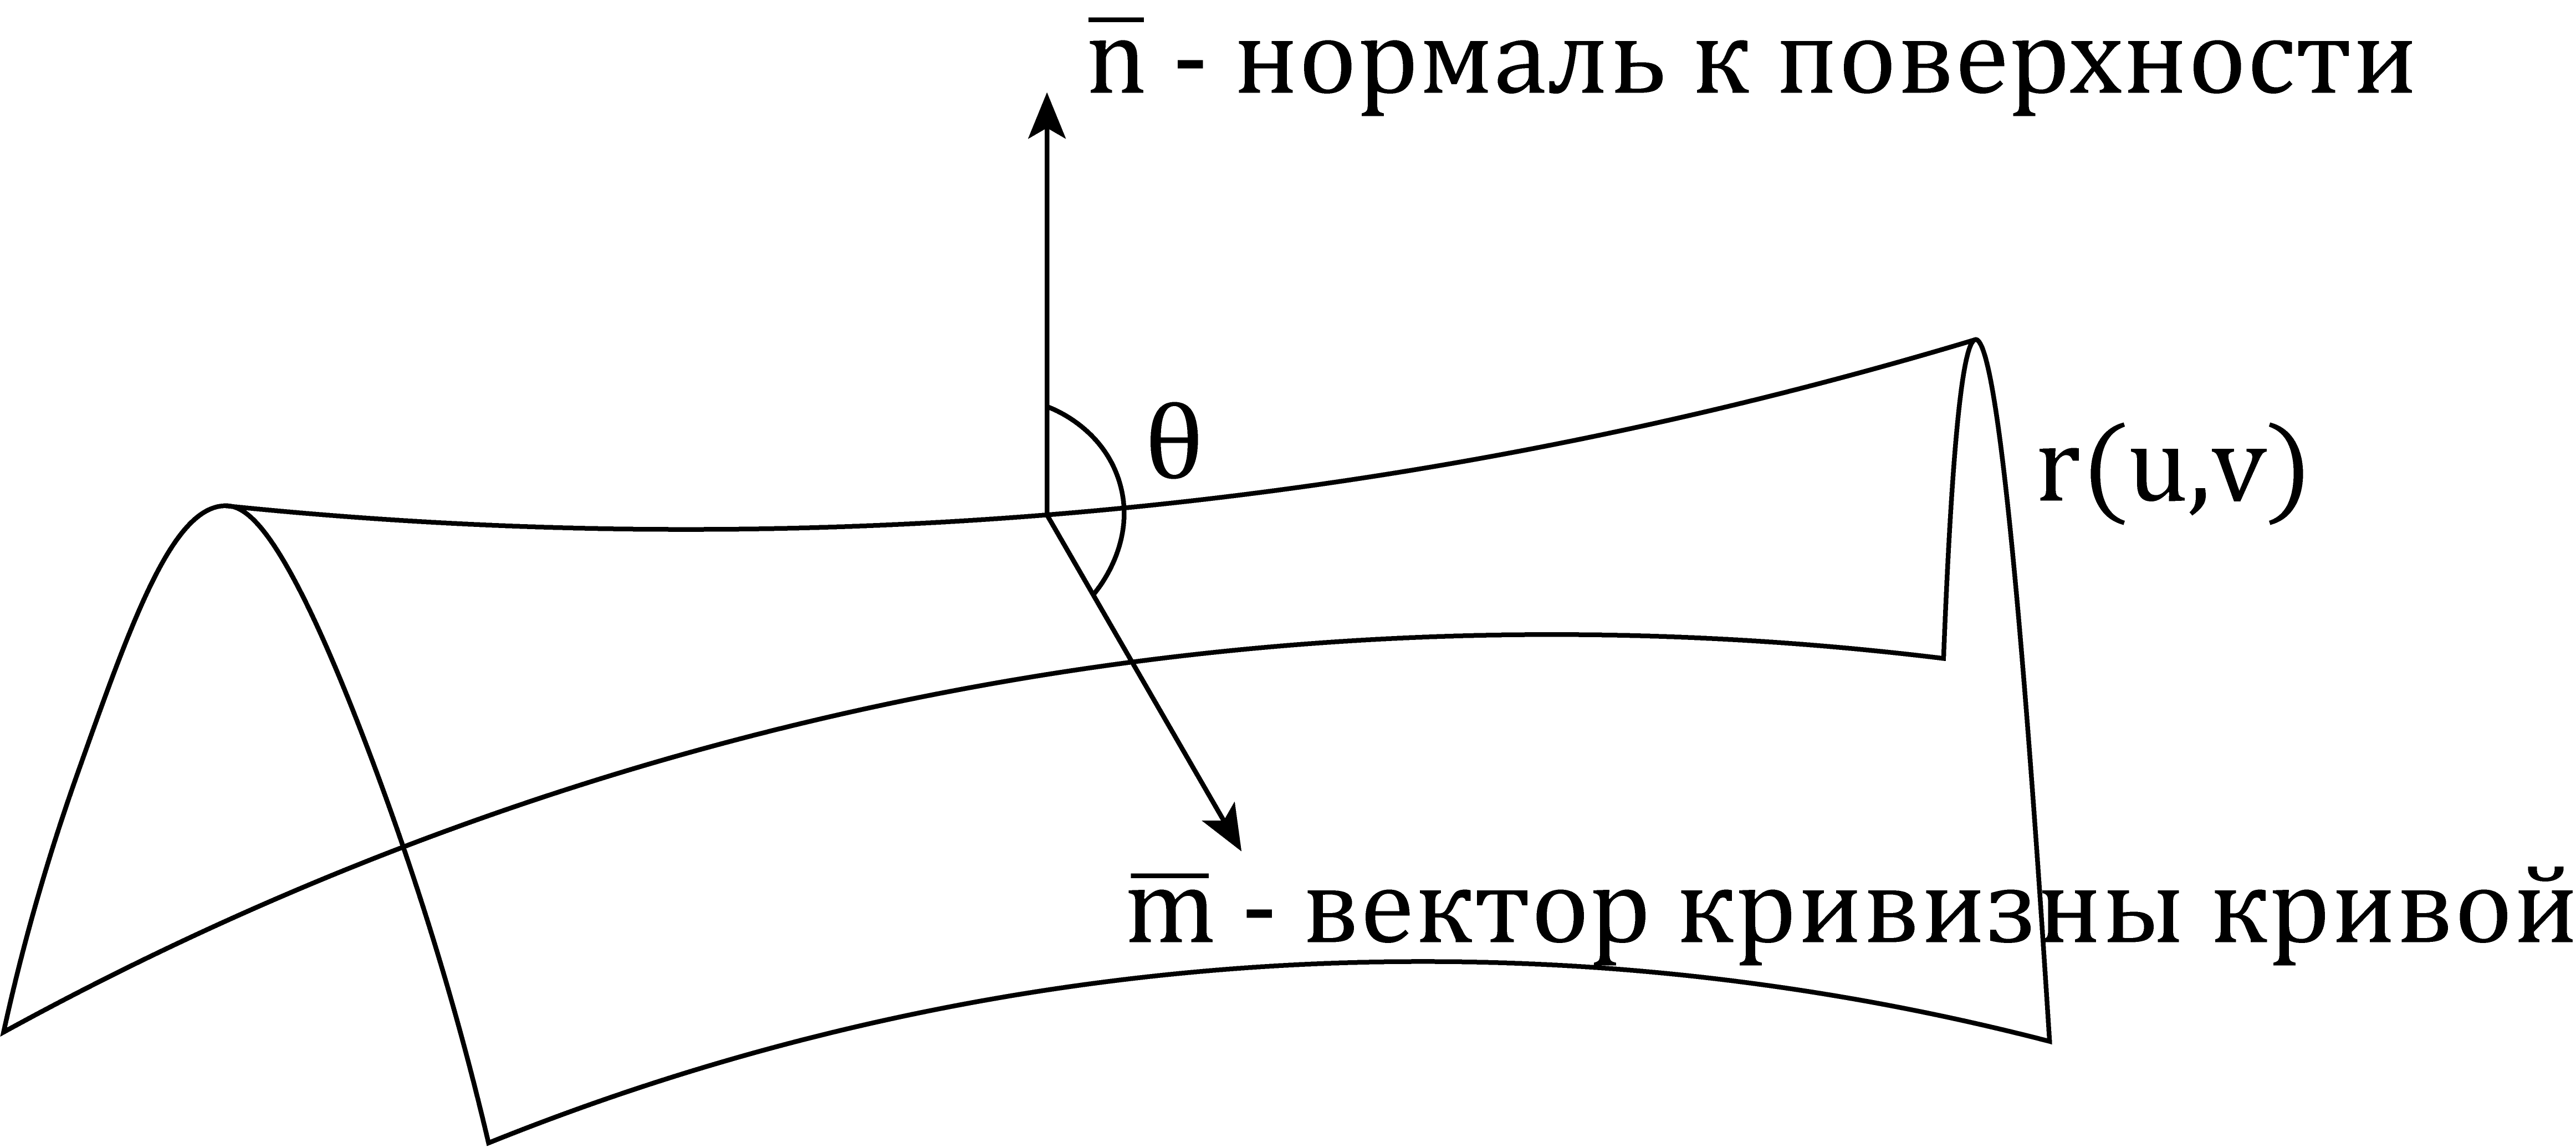
\includegraphics[width=10cm]{pics/7_5.png}
	\end{figure}
	\[\psi(s) \qq k = |\os{=\ol{m}}{\psi''(s)}|\]
	\[\theta \text{ --- угол между $\ol{m}$ и $\ol{n}$}\]
	\[k = |\psi''(s)| = \dfrac{\ol{\psi}''(s) \cdot \ol{n}}{\cos \theta}\]
	\[u(s),\ v(s) \text{ --- внутр. ур-я кривой}\]
	\[\psi' = r_u u' + r_v v'\]
	\[\psi'' = \ol{r}_{uu} u'^2 + \ol{r_{uv}} u' v' + \ol{r}_u u'' + \ol{r}_{uv} u' v' + \ol{r}_{vv} v'^2 + \ol{r}_v v''\]
	\[\ol{r}_u \ol{n} = 0\]
	\[\ol{r}_v \ol{n} = 0\]
	\[\RA \psi'' n = \ol{r}_{uu} \ol{n} u'^2 + 2 \ol{r}_{uv} n u'v' + \ol{r}_{vv} n v'^2\]
	Пусть $L,\ M,\ N$ --- соответств. $u',\ v'$ коэф., тогда:
	\[\psi'' n = L u'^2 + 2 M u'v' + N v'^2 := \RNumb{2}(u',\ v')\]

	\begin{Reminder}
		\[\RNumb{1}(u',v') = E u'^2 + 2 F u' v' + G v'^2\]
	\end{Reminder}

	\begin{theorem}
		Если s --- нат. параметризация, $k \cos \theta = \RNumb{2} (u'(s),\ v'(s))$
	\end{theorem}

	\begin{theorem}
		$\forall$ параметризации $\Ra k \cos \theta = \dfrac{\RNumb{2} (u'(t); v'(t))}{\RNumb{1} (u'(t); v'(t))}$
	\end{theorem}
	\begin{proof}
		Пусть теперь $\psi(t)$ --- произвольная параметризация
		\[\psi'(s) = \dfrac{\varphi'(t)}{|\varphi'(t)|}\]
		\[(u'(s), v'(s)) = \dfrac{(u'(t), v'(t))}{|\varphi'(t)|}\]
		\[|\varphi'(t)| = E u'^2(t) + 2F u'(t) v'(t) + G v'^2(t)\]
		\[k \cos \theta = \dfrac{\RNumb{2} (u'(t),\ v'(t))}{|\varphi'(t)|} = \dfrac{\RNumb{2} (u'(t); v'(t))}{\RNumb{1} (u'(t); v'(t))}\]
	\end{proof}

	\begin{Example}
		\[\begin{cases}
			x = R \cos \varphi \cos \psi\\
			y = R \sin \varphi \cos \psi\\
			z = R \sin \psi
		\end{cases} \text{ --- сфера}\]
		\begin{figure}[H]
			\centering
			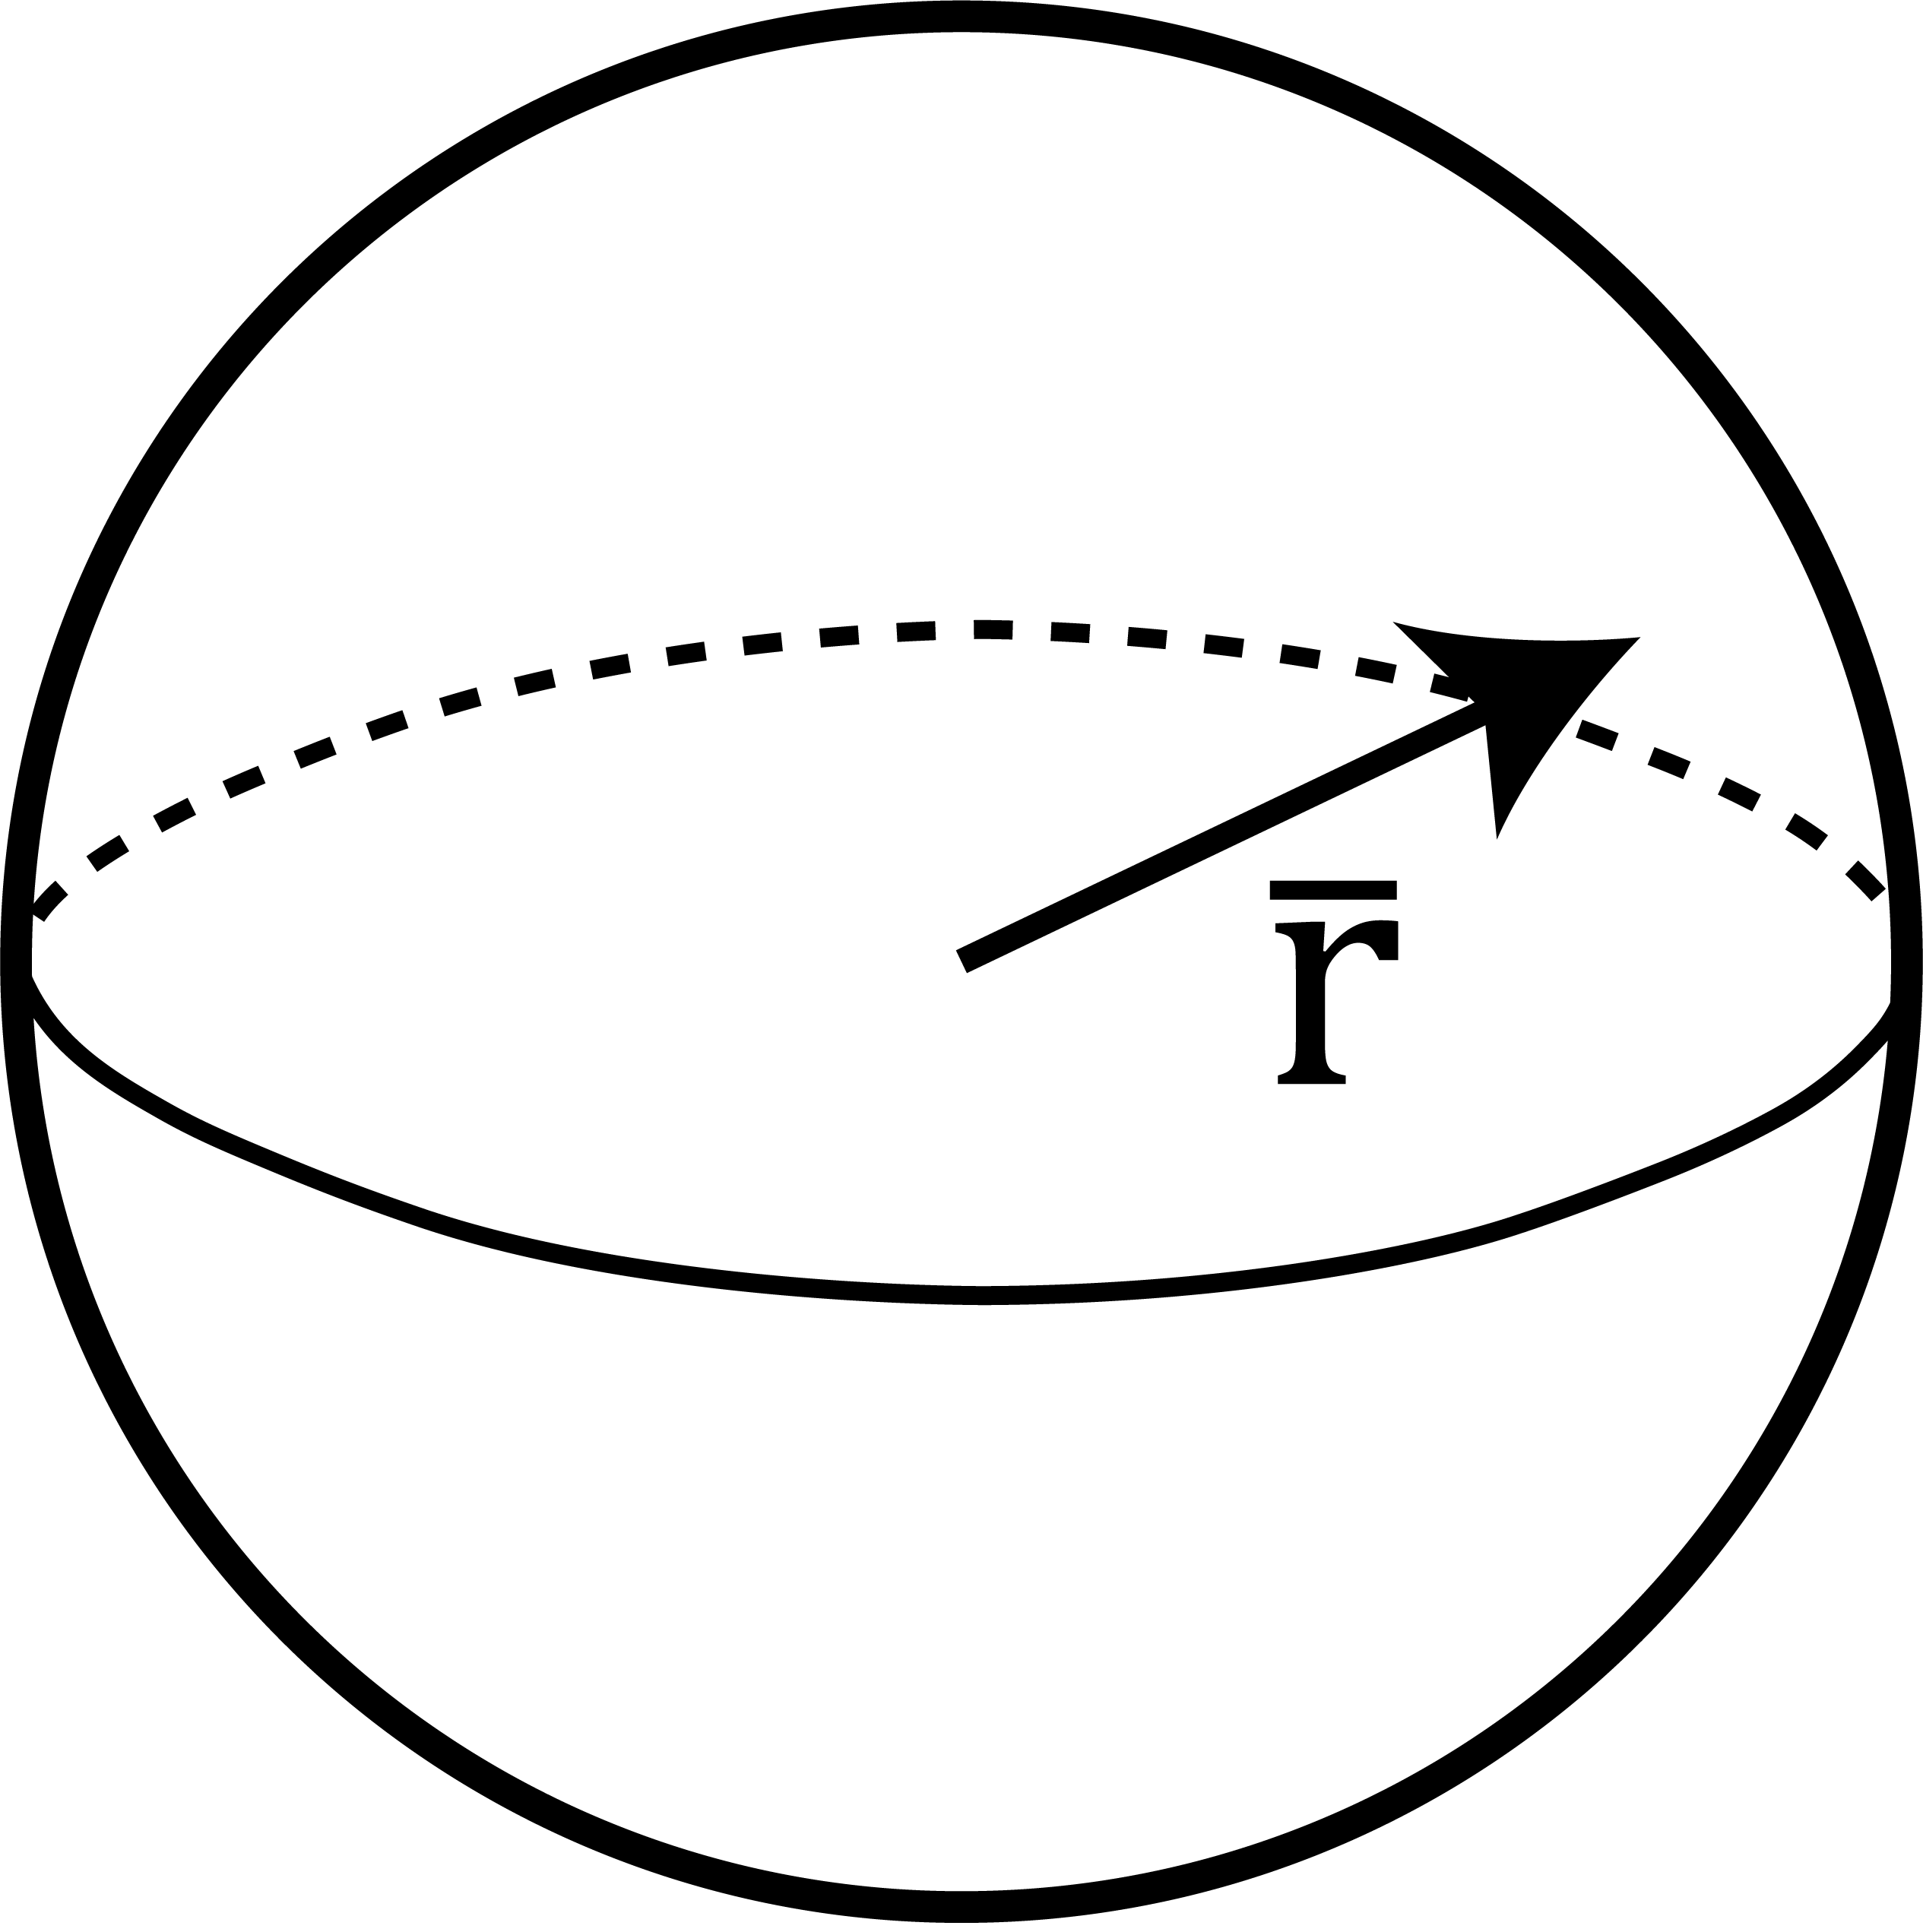
\includegraphics[width=4cm]{pics/7_6.png}
		\end{figure}
		\[\ol{n} = \dfrac{\ol{r}}{R} = (\cos \varphi \cos \psi,\ \sin \varphi \cos \psi,\ \sin \psi)\]
		\[\ol{r}_{\varphi \varphi} = (-R \cos \varphi \cos \psi,\ -R \sin \varphi \cos \psi,\ 0)\]
		\[L = -R \cos^2 \psi\]
		\[\ol{r}_{\varphi \psi} = (R \sin \varphi \sin \psi,\ -R \cos \varphi \sin \psi,\ 0)\]
		\[M = 0\]
		\[\ol{r}_{\psi \psi} = (-R \cos \varphi \cos \psi,\ -R \sin \varphi \cos \psi,\ -R \sin \psi)\]
		\[N = -R\]
	\end{Example}

	\subsection{Теорема Мёнье}
	\begin{advice}
        Посмотреть формулировку в учебнике Александрова и Нецветаева
    \end{advice}
	\begin{figure}[H]
		\centering
		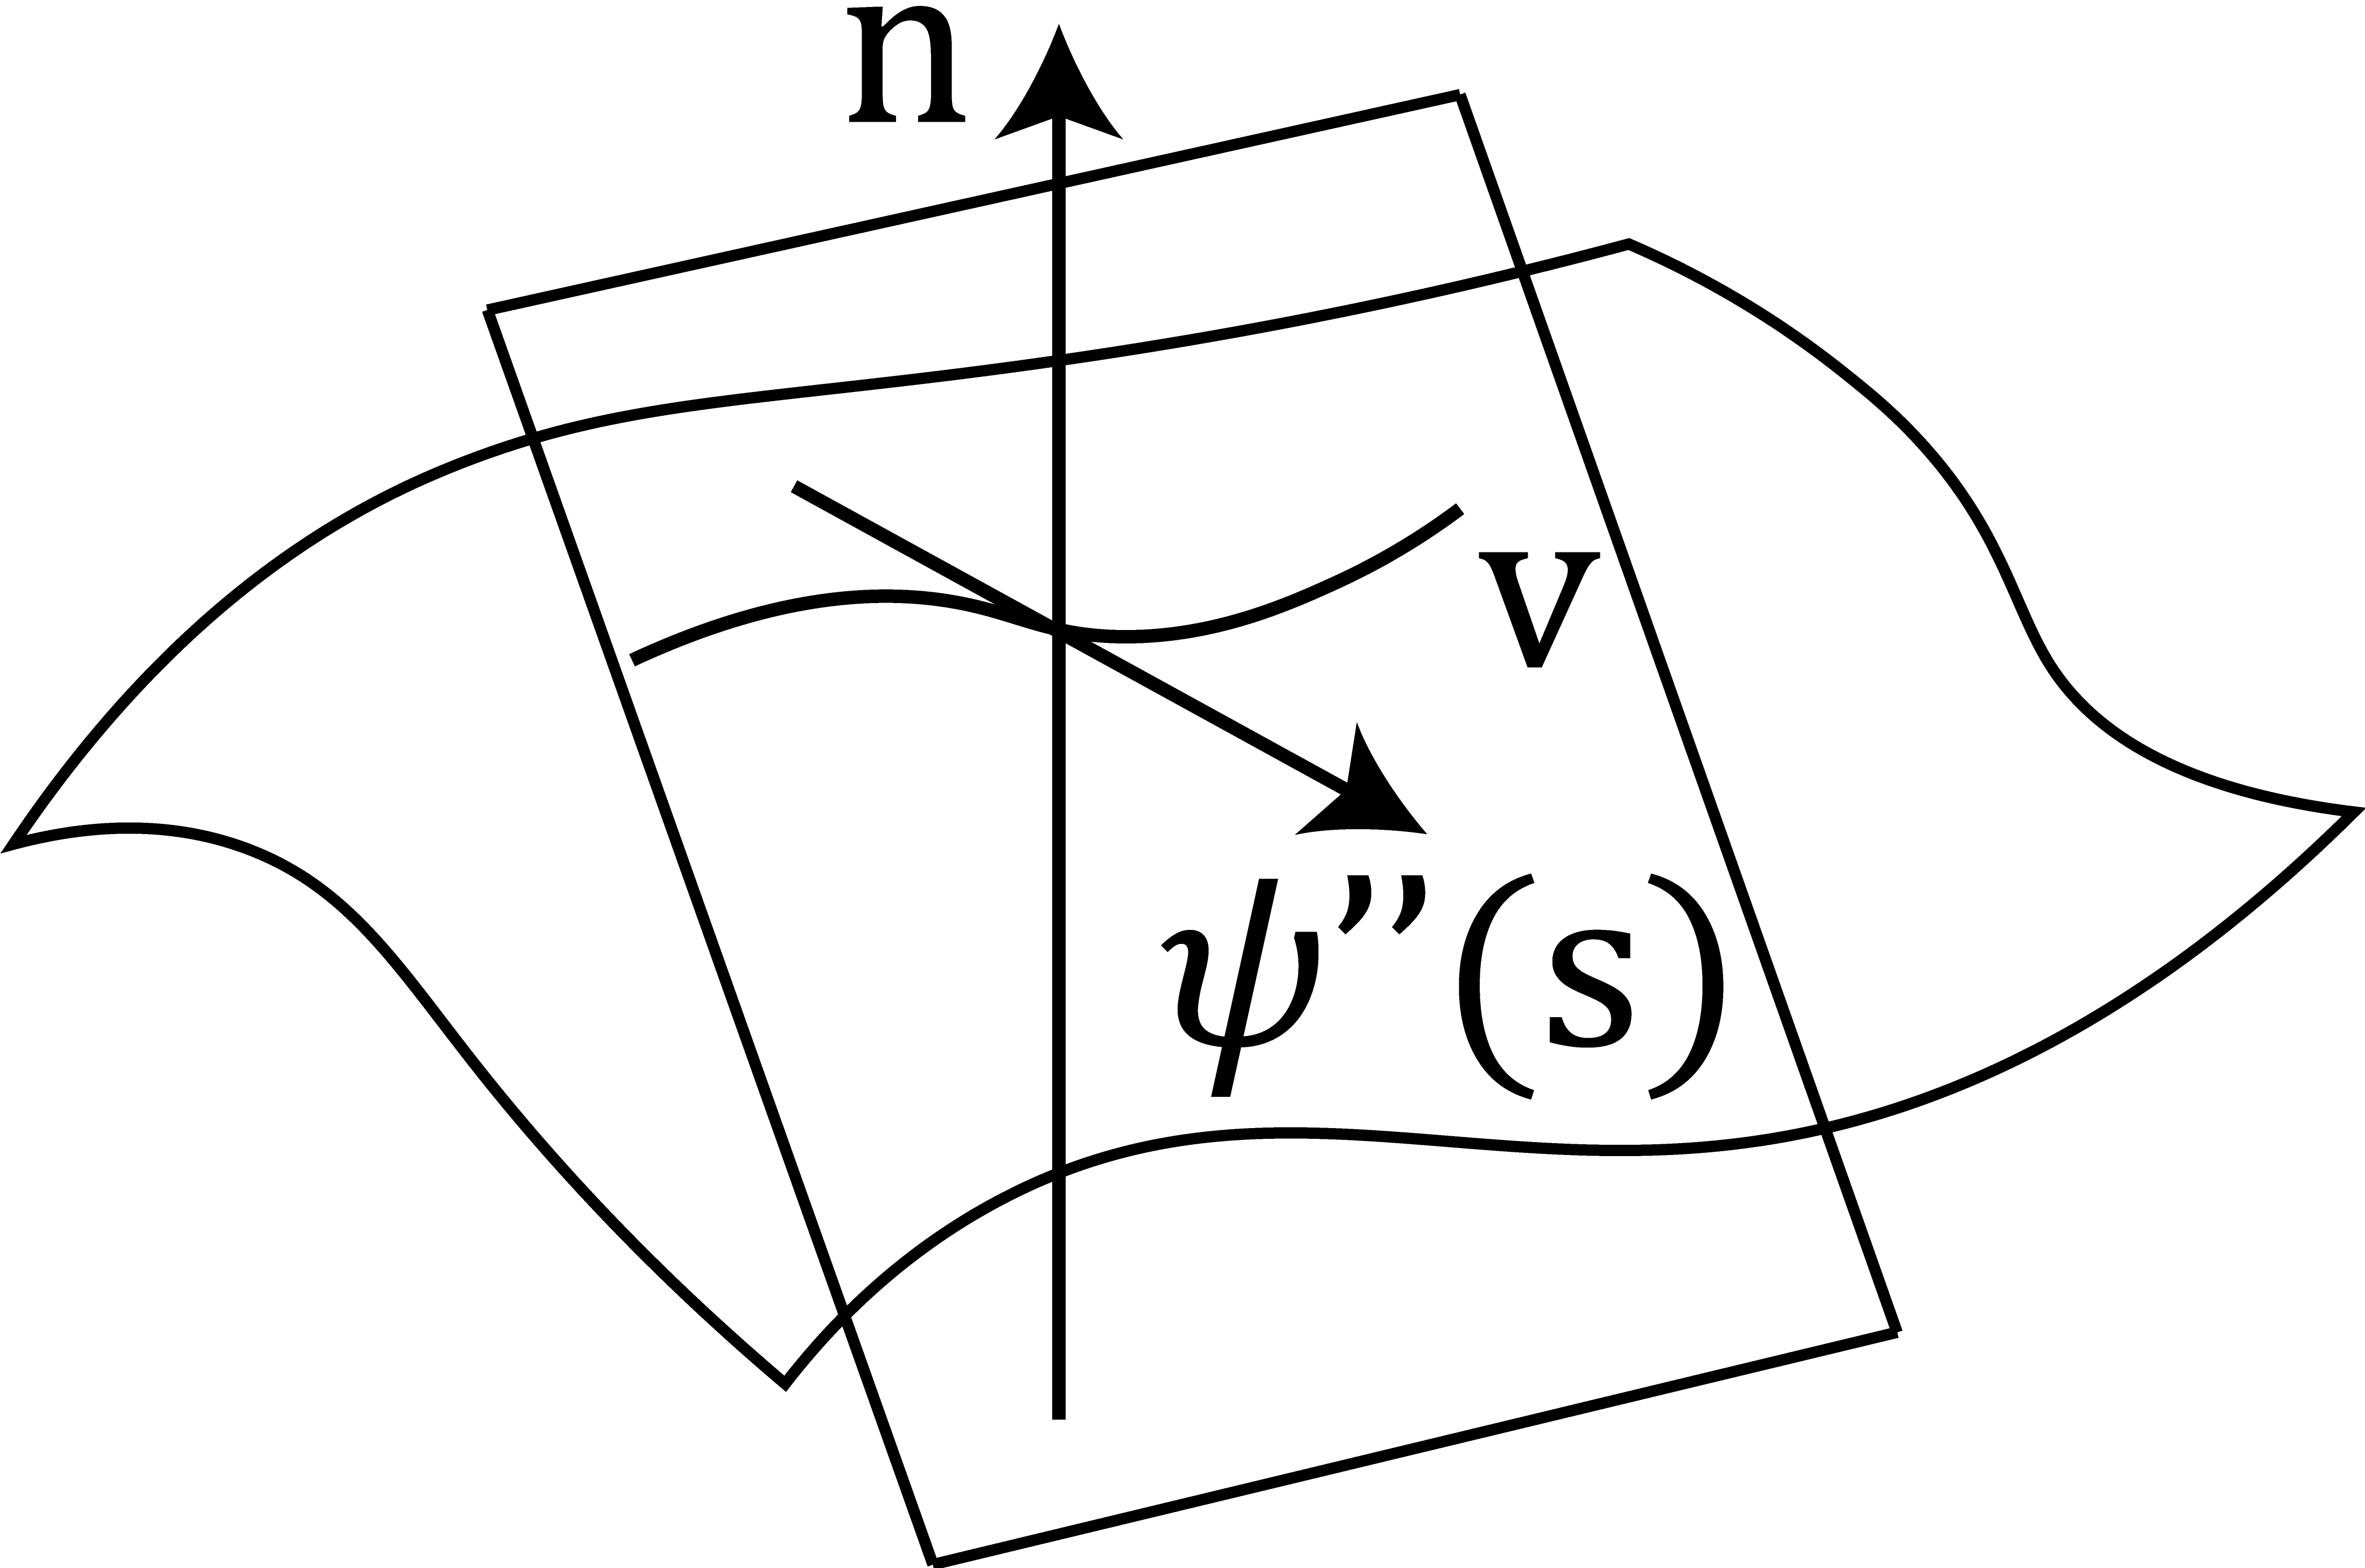
\includegraphics[width=7cm]{pics/7_7.png}
	\end{figure}
	\begin{theorem}[Мёнье?]
		Проекция векторов кривизны кривых на поверхности с данным касательным вектором на вектор нормали к поверхности одинаковы (все это $k \cos \theta$)
	\end{theorem}
	$(u'(s_0),\ v'(s_0)) \text{ --- у всех таких кривых одинак.}$
	\begin{figure}[H]
		\centering
		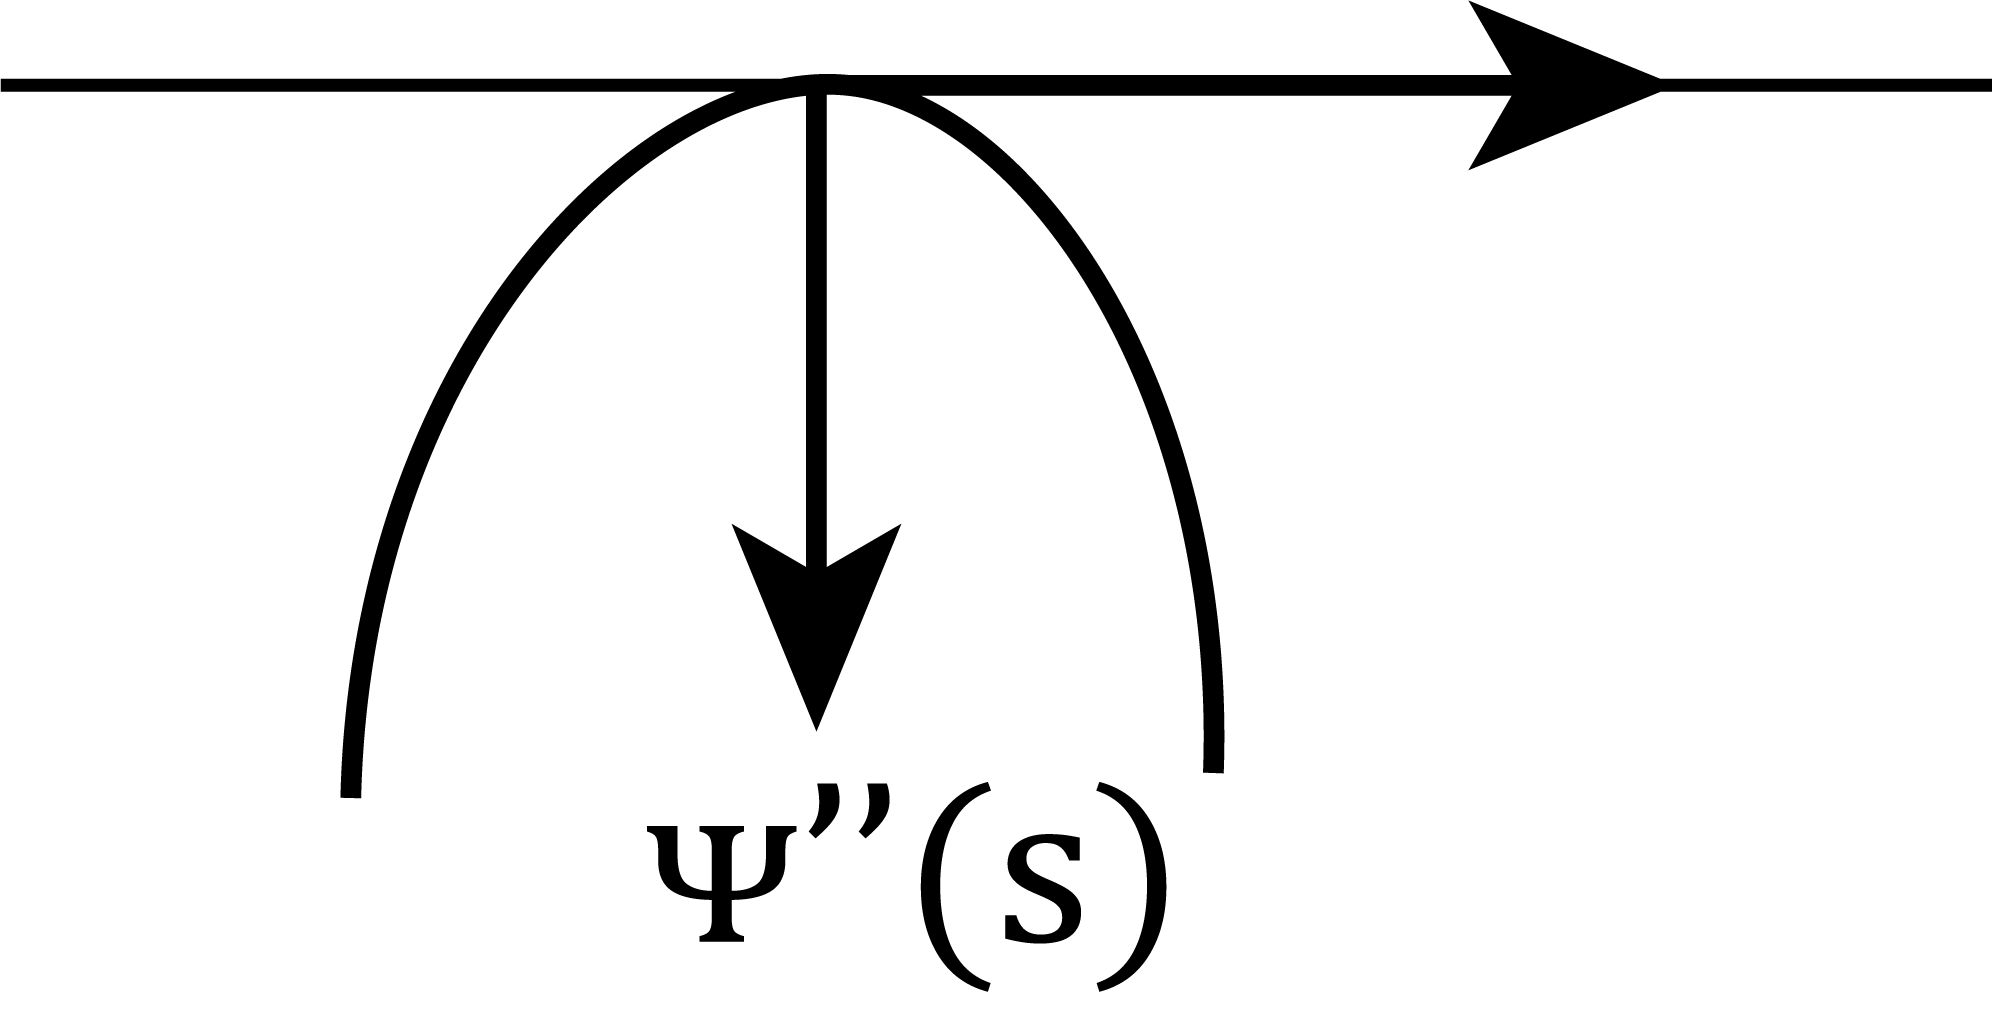
\includegraphics[width=4.5cm]{pics/7_8.png}
	\end{figure}

	\begin{Theorem}[Мёнье?]
		\[k \cos \theta = \RNumb{2}(u'(s),\ v'(s)), \text{ если s --- натур. параметризация}\]
	\end{Theorem}

	\begin{proof}
		Пусть параметризации натуральные
	\end{proof}

	Возьмем кривую: $\cos \theta = \pm 1$ (знак зависит от $\ol{n}$)\\
	Рассмотрим кривые с данным единичным кас. векором и $\cos \theta = \pm 1 \Ra$ у них одинаковые кривизны
	\[k_{\triangledown} = \RNumb{2}(u'(s),\ v'(s))\]
	Нормальная кривизна поверхности в направлении $\triangledown$
\end{document}
